\documentclass{article}
\usepackage{amsmath}
\usepackage{geometry}[a4paper]
\usepackage{graphicx}
\graphicspath{ {../../figures/} }
\usepackage{enumerate}
\usepackage{microtype}
\usepackage{hyperref}
\usepackage{subcaption}

\title{Reports of Recent Works}
\author{Kai Chen}
\date{Jan. 14, 2018}

% \tableofcontent
\begin{document}
	\maketitle
	\section{Mutual information between Gaussian random variables}
	Here I am going to derive the expression for mutual information between two variables generated by random processes analytically. Let's define ${X_n}$ and ${Y_n}$ as:
	\begin{equation}
		\begin{aligned}
			&X_n = \alpha X_{n-1} + \epsilon_n \\
			&Y_n = \beta Y_{n-1} + \xi_{xy}f(X_{n - 1}) + \eta_n
		\end{aligned}
	\end{equation}
	where $\epsilon_n$ and $\eta_n$ are independent random variables with normal distribution, and $\alpha$, $\beta$ and $\xi_{xy}$ are the self interaction strength and cross interaction strength between \{X\} and \{Y\}, respectively. $f(X)$ is a functional mapping, which could be either linear or nonlinear.
		\subsection{Derivations}
		I will mainly discussed the first order correlation between $X_n$ and $Y_{n+1}$, connected by linear function, i.e. $f(X) = X$ is a linear function, in terms of mutual information.
		\begin{equation}
			\begin{aligned}
				&X_n = \alpha X_{n-1} + \epsilon_n \\
				&Y_{n+1} = \beta Y_{n} + \xi f(X_n) + \eta_{n+1}
			\end{aligned}
		\end{equation}
		I would like to write down the expression of mutual information as a function of $\xi$. $X$ and $Y$ stand for $X_n$ and $Y_{n+1}$ for convenience below.
		\begin{equation}
			\begin{aligned}
				I(X;Y) & = \sum_X\sum_Yp(x,y)log\frac{p(x,y)}{p(x)p(y)} \\
				& = H(X) + H(Y) - H(X,Y)
			\end{aligned}
		\end{equation}
		where p(x,y) is the joint probability distribution of X and Y, and p(x) and p(y) is the probability density function of variable X and Y. H is entropy. Since $\epsilon_i$ and $\eta_i$ are independent Gaussian random variables, it is easy to conclude that X and Y are Gaussian distributed. By substuting p(x) into the function of entropy.
		\begin{equation}
			H(X) = \int p(x)log(p(x)) = \frac{1}{2}(1+log(2\pi\sigma_x^2))
		\end{equation}
		where $\sigma_x$ is the standard deviation of X. The entropy of Y, H(Y), can be expressed in the same way. Define the correlation coefficient between X and Y is $\rho$, the joint entropy of X and Y can be expressed as:
		\begin{equation}
			H(X,Y) = \int p(x,y)log(p(x,y)) = 1+log(2\pi\sigma_x\sigma_y\sqrt{1-\rho^2})
		\end{equation}
		By substituting them into the expression of mutual information, we can obtain the expression of mutual information in the bivariate Gaussian distributed case as,
		\begin{equation}
			I(X,Y) = -\frac{1}{2}log(1-\rho^2)
		\end{equation}
		Then, we need to calculate the correlating coefficient $\rho$,
		\begin{equation}
			\rho = \frac{Cov(x,y)}{\sigma_x\sigma_y} = \frac{E[XY] - \mu_x\mu_y}{\sigma_x\sigma_y}
		\end{equation}
		Calculate the E(X), E(Y), $\sigma_x$ and $\sigma_y$.
		\begin{equation}
			E[X_n] = E[\alpha X_{n-1}+\epsilon_n] = E[\sum^n_{i=1}\alpha^{n-i}\epsilon_i]=\sum^n_{i=1}\alpha^{n-i}E[\epsilon_i] = 0
		\end{equation}
		\begin{equation}
			E[Y_{n+1}] = E[\beta Y_{n}+\xi X_n + \eta_{n+1}] = E[\sum^{n +1}_{i=1}\beta^{n+1-i}\eta_i +\xi\sum^{n}_{i=1}\beta^{n-i}\sum^{i}_{j=1}\alpha^{i-j}\epsilon_j] = 0
		\end{equation}
		\begin{equation}
			\begin{aligned}
				D[X] & = D[\sum^n_{i=1}\alpha^{n-i}\epsilon_i] = \sum^n_{i=1}\alpha^{2(n-i)}D[\epsilon_i] = \frac{1 - \alpha^{2n}}{1-\alpha^2}
			\end{aligned}
		\end{equation}
		\begin{equation}
			\begin{aligned}
				D[Y] & = D[\sum^{n +1}_{i=1}\beta^{n+1-i}\eta_i +\xi\sum^{n}_{i=1}\beta^{n-i}\sum^{i}_{j=1}\alpha^{i-j}\epsilon_j] \\
				& = \sum^{n + 1}_{i=1}D[\beta^{n - i + 1}\eta_i] +\xi^2D[\sum^{n}_{i=1}\beta^{n-i}\sum^{i}_{j=1}\alpha^{i-j}\epsilon_j]
			\end{aligned}
		\end{equation}
		If $\alpha = \beta$,
		\begin{equation}
			D[Y] = \frac{1 - \alpha^{2n+1}}{1-\alpha^2} + \xi^2\sum^{n-1}_{i=0}(j+1)^2\alpha^{2i}
		\end{equation}
		If $\alpha\neq\beta$,
		\begin{equation}
			D[Y] = \frac{1 - \beta^{2n+1}}{1-\beta^2} + \xi^2\sum^{n}_{i=1}(\frac{\beta^i - \alpha^i}{\beta - \alpha})^2
		\end{equation}
		By definition, standard deviations of X and Y are square roots of their deviation. Eventually, we need to calculate E(XY).
		\begin{equation}
			E[XY] = E[(\sum^n_{i=1}\alpha^{n-i}\epsilon_i)(\sum^{n +1}_{i=1}\beta^{n+1-i}\eta_i +\xi\sum^{n}_{i=1}\beta^{n-i}\sum^{i}_{j=1}\alpha^{i-j}\epsilon_j)]
		\end{equation}
		The first part of right side of the equation above is zero, since $\epsilon_i$ and $\eta_i$ are independent. And $E[\epsilon_i\epsilon_j] = \delta_{ij}$. So when $\alpha = \beta$,
		\begin{equation}
			E[XY] =	\frac{\xi}{1-\alpha^2}(\frac{1-\alpha^{2n}}{1-\alpha^2} - n\alpha^{2n})
		\end{equation}
		When $\alpha\neq\beta$,
		\begin{equation}
			E[XY] =	\frac{\xi}{1-\alpha/\beta}(\frac{1-(\alpha\beta)^n}{1-\alpha\beta} - \frac{1-\alpha^{2n}}{1-\alpha^2}\frac{\alpha}{\beta})
		\end{equation}

		When $n >> 1$, we can substitute E(XY), $\mu_x$, $\mu_y$, $\sigma_x$ and $\sigma_y$ into $\rho$. For $\alpha = \beta$,
		\begin{equation}
			\rho^2 = \frac{\xi^2}{(1-\alpha^2)^2 + \xi^2(1+\alpha^2)}
		\end{equation}
		for $\alpha\neq\beta$,
		\begin{equation}
			\rho^2 = \frac{\xi^2(1-\beta^2)}{(1-\alpha\beta)^2(1-\alpha^2) + \xi^2(1-(\alpha\beta)^2)}
		\end{equation}

		\subsection{Numerical Sample}
		Here, I presented results from numerical simulations. Both the theoretical and numerical value of the mutual information as the function of interacting strength are ploted.
		\begin{figure}[h]
			\centering
			\begin{subfigure}[b]{0.3\textwidth}
				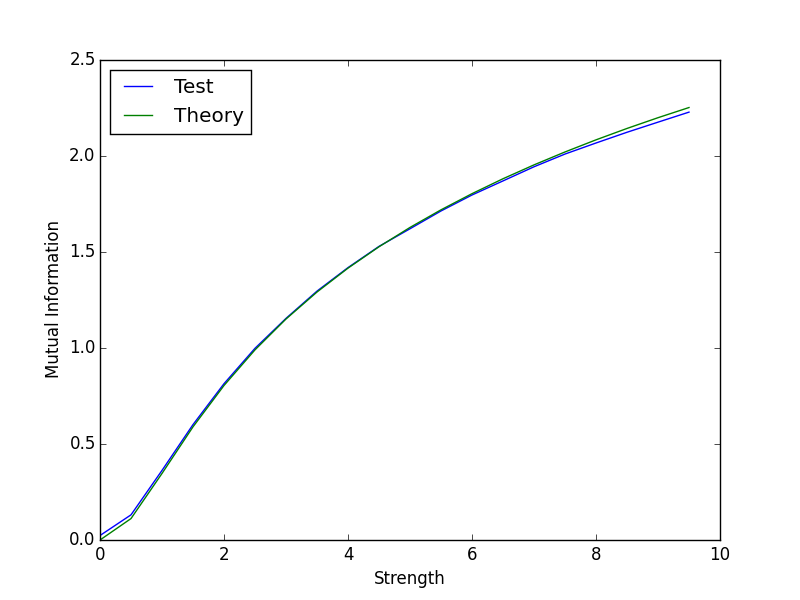
\includegraphics[width = \textwidth]{gauss/linear_001_001_150.png}
				\caption{$\alpha = 0.01$, $\beta = 0.01$.}
			\end{subfigure}
			\begin{subfigure}[b]{0.3\textwidth}
				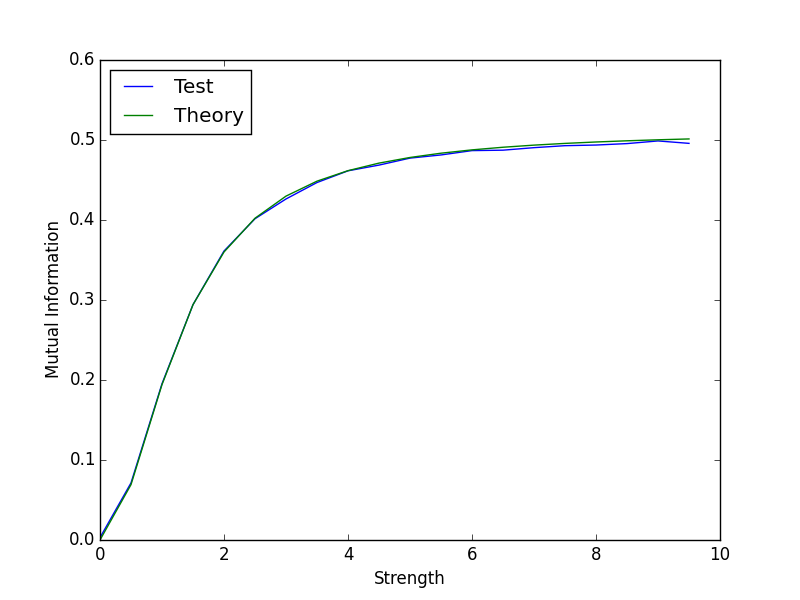
\includegraphics[width = \textwidth]{gauss/linear_001_06_50.png}
				\caption{$\alpha = 0.01$, $\beta = 0.6$.}
			\end{subfigure}
			\begin{subfigure}[b]{0.3\textwidth}
				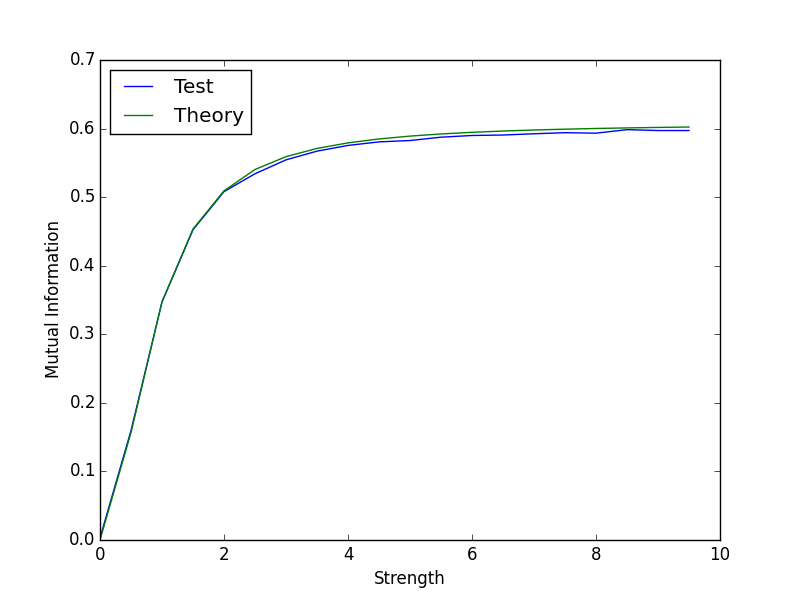
\includegraphics[width = \textwidth]{gauss/linear_05_06_50.png}
				\caption{$\alpha = 0.5$, $\beta = 0.6$.}
			\end{subfigure}
		\end{figure}

	\section{Two neuron system}
		In order to reduce the difficulty of analysis, I decided to start with two neuron system raster than one to multi neuronal system. By increasing the length of simulation period ten times, we can roughly simulate cases which is equivilant to one to ten neurons interaction neglecting spatial distribution of neurons.
		% In two-neuron system, I can manipulate the noise level by adjusting the rate of feed Poisson driving rate
		Here, I give the neuronal network setting applied in my simulation.
		\begin{tabular}{c|c}
			\hline
			Driving rate & 1.5 $ms^{-1}$\\
			\hline
			Driving strength & 0.005 \\
			\hline
			Synaptic strength(Excitatory)& 0.005 \\
			\hline
			Simulation time & 60 s\\
			\hline
			Timing step & 1/32 ms \\
			\hline
		\end{tabular}
		\subsection{Autocorrelating time scale}
			According to the requirement of wide-sense stationary process, the mean and autocovariane do not vary respect to time. Therefore, I ran two-neuron system to obtain 800 trials. The means and standard deviations of spike train and LFP at each time point were measured. Here, the standard deviation stands for autocovariance between $X_n$ and itself.
			% \begin{figure}[ht]
			% 	\centering
			% 	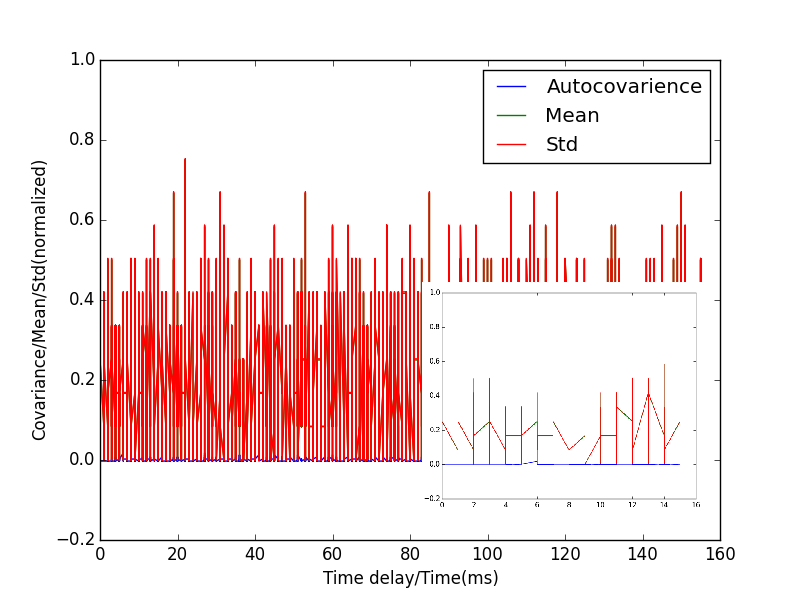
\includegraphics[scale = 0.5]{n1sb_comb.png}
			% 	\caption{Stationary tests for spike train of presynaptic neuron. autocovariance(blue), mean value(green) and standard deviation(red) are plotted, respectively.}
			% 	\label{fig:spike_auto}
			% \end{figure}
			As for spike train of presynaptic neuron, I take the time step as 0.5 milliseconds, which means that the element in spike train series is "1" if there is a spiking events within 0.5 ms time window, and is "0" otherwise. From Figure \ref{fig:spike_auto}, I find that the auto correlation length of spike train is almost zero.
			% \begin{figure}[ht]
			% 	\centering
			% 	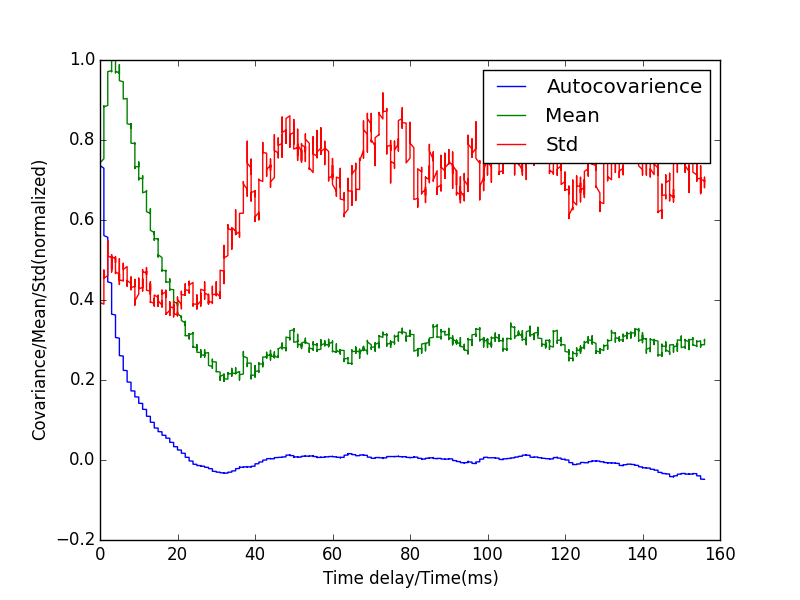
\includegraphics[scale = 0.5]{n2i.png}
			% 	\caption{Stationary tests for LFP series of postsynaptic neuron. autocovariance(blue), mean value(green) and standard deviation(red) are plotted, respectively.}
			% 	\label{fig:lfp_auto}
			% \end{figure}
			In Figure \ref{fig:lfp_auto}, the mean and standard deviation of signal reach their stationary state, respectively. Therefore, I take data in the first 40 milliseconds away, and calculate its autocovariance. The length of autocorrelation is around 20 milliseconds.

		\subsection{Choise of time step in MI calculation}
			After running test under different timing steps, I decided to choose 0.5 ms as the proper step. If smaller steps are taken, '1' elements is far too less than '0'. In this way, the signal peak of mutual information would be barried into noise level.

		\subsection{Correlation interacting strength and mutual information}
			% \begin{figure}[ht]
			% 	\centering
			% 	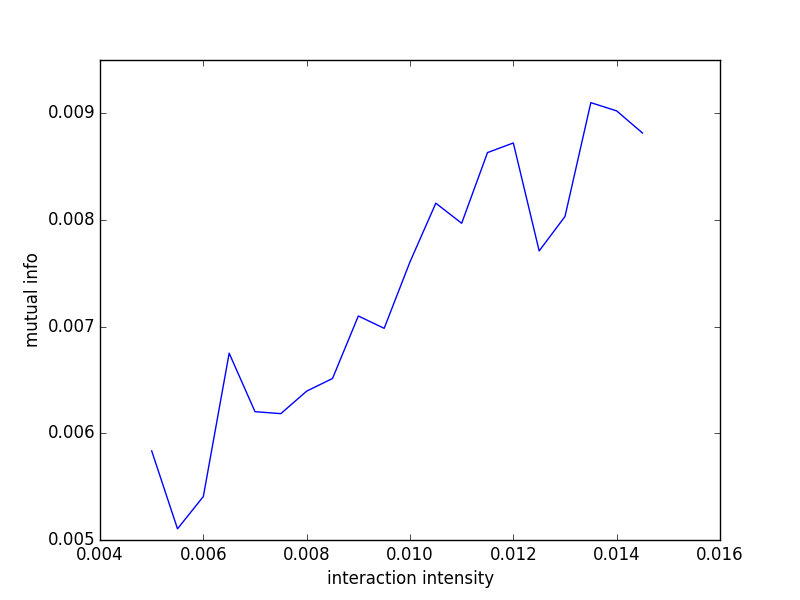
\includegraphics[scale = 0.5]{oct7.png}
			% 	\caption{Relationship between synaptic strength and the peak of mutual information.}
			% 	\label{fig:relation}
			% \end{figure}
		% \subsection{Proposal for theoretical explanations}
\end{document}
